\chapter{\label{a3-extractors}Charge Extractor Investigations}

\minitoc

\notes[inline,caption={}]{
	\section{Plan}
	\subsection{Topics}
	\begin{itemize}
		\item RMS extracted charge with varying integration window size and shift with different NSBs and amplitudes (and combination of amplitudes)
		\item Charge resolution of different methods with different NSB (including full integration method)
		\item in the absence of the need for peak finding (laser illumination), and when peak finding is important (Cherenkov) - split into two, best integration technique (different NSBs, different integration window sizes), and best peak finding (different NSBs, need Cherenkov data)
		\item window size might actually change for Cherenkov - got to capture entire signal, and signal might not be centred at "calculated peak time".
	\end{itemize}
	\subsection{Questions}
	\begin{itemize}
		\item ?
	\end{itemize}
}

\section{Introduction}

In Chapter~\ref{ch6-reduction}, the different algorithms for extracting charge from a waveform is extensively discussed, as well as the important considerations one must be vigilant of. This Appendix is provided to inform about the performance of the chosen charge extraction approaches, \textit{Cross Correlation} and \textit{Neighbour Peak Finding}, in comparison to typical charge extraction approaches, in the context of \gls{chec-s}.

\section{Integration Window}

\begin{figure}
  \begin{subfigure}[b]{0.49\textwidth}
    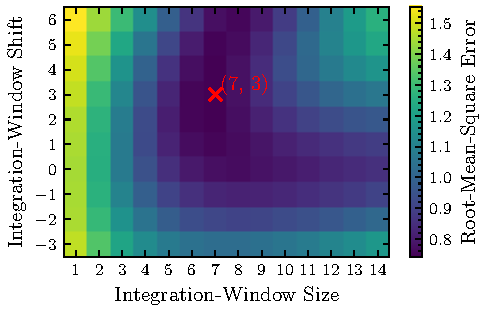
\includegraphics[width=\textwidth]{amp1nsb5}
    \caption{1~p.e. illumination, 5~MHz noise.}
    \label{fig:amp1nsb5}
  \end{subfigure}
  \hfill
  \begin{subfigure}[b]{0.49\textwidth}
    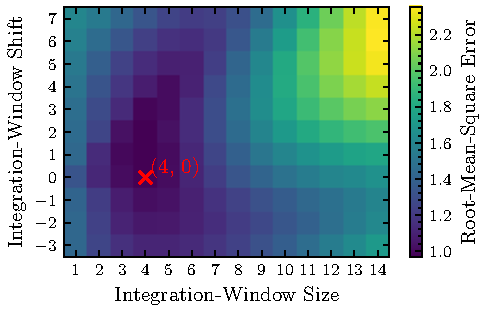
\includegraphics[width=\textwidth]{amp1nsb125}
    \caption{1~p.e. illumination, 125~MHz noise.}
    \label{fig:amp1nsb125}
  \end{subfigure}
  \hfill
  \begin{subfigure}[b]{0.49\textwidth}
    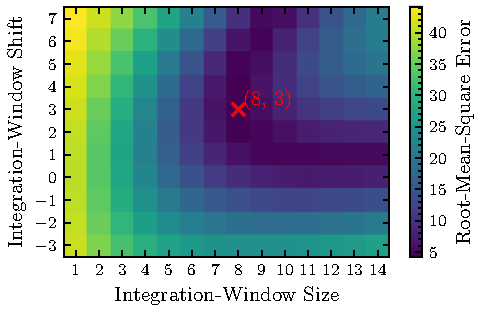
\includegraphics[width=\textwidth]{amp50nsb5}
    \caption{50~p.e. illumination, 5~MHz noise.}
    \label{fig:amp50nsb5}
  \end{subfigure}
  \hfill
  \begin{subfigure}[b]{0.49\textwidth}
    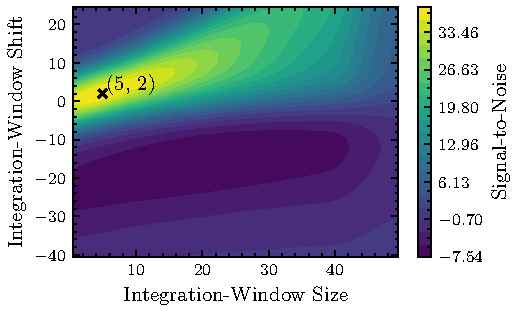
\includegraphics[width=\textwidth]{amp50nsb125}
    \caption{50~p.e. illumination, 125~MHz noise.}
    \label{fig:amp50nsb125}
  \end{subfigure}
  \caption[Optimal integration window parameters.]{Root-mean-square error as a function of window width and shift, for different amplitudes and noise values. The minimum, highlighted with the red annotation, indicates the optimal parameters for an integration window applied to a CHEC-S waveform. The extracted charges are not corrected for integration window size in these figures.}
  \label{fig:rmse_noc}
\end{figure}

As an alternative to the \textit{Cross Correlation} integration approach, one may instead use a simple integration window, defined by the number of samples inside the ``window width'', and the number of samples the window is ``shifted'' by from the peak time. In order to perform investigations using the performance of the integration window approach, one must first find the optimal values for the width and shift of the window when extracting charge from a \gls{chec-s} waveform. This exercise was performed using a Monte Carlo simulation of the lab set-up, where the camera was uniformly illuminated. As the pulse time is consistent in simulations of this nature, it allows the investigation to be solely on the integration approach, avoiding the interference from peak finding.

As explained in Chapter~\ref{ch6-reduction}, the optimal integration window parameters are noise dependant; a larger integration window is likely to include more noise (\gls{nsb} and \gls{dcr}). It also stands to reason that at higher signal illuminations, the impact of noise on the charge extraction is diminished. In Figure~\ref{fig:rmse_noc} the \gls{rmse} as a function of integration window parameters is shown for different amplitudes and noise values. The \gls{rmse} is calculated using Equation~\label{eq:charge_res}, where the true charge is the direct value measured by the photosensor, extracted from the Monte Carlo file. No attempt was made to correct for the signal outside of the integration window range for the results in Figure~\ref{fig:rmse_noc}. As a result, the conflict between a large window size to contain the full signal, and a small window to minimise noise is evident. In conclusion, an integration window width of 8 samples and a shift of 3 samples appears to be optimal for all cases, apart from the low-amplitude high-noise case (Figure~\ref{fig:amp1nsb125}), where a smaller window of 4 samples is preferred, with a shift of 1 sample. 

If we instead


\change[inline]{Same discriminator used for different NSB}



